\smalltitle{سوال 2}
\\\noindent
در ابتدا به چند نکته اشاره می‌کنم که لازم بود در کد این سوال رعایت کنم.
در ابتدا برای استفاده از تابع
\lr{pthread\_attr\_setaffinity\_np}
مجبور بودم که در اولین خط برنامه قبل از
\lr{import}ها
خط
\lr{\#define \_GNU\_SOURCE}
را اضافه کنم.
\link{https://stackoverflow.com/a/7269859/4213397}{منبع}
تابع مذکور به ما اجازه می‌دهد که مشخص کنیم که هر ریسمان بر روی کدام هسته‌های
\lr{CPU}
قابل اجرا باشد.

یکی دیگر از مشکلاتی که وجود داشت نیازمندی به
align
کردن مموری به
\lr{page}های
سیستم بود. بدین منظور که به عنوان مثال در سیستم من که سایز صفحات 4096 بایت است،‌ اول مموری که
به تابع
\lr{mprotect}
داده می‌شود باید بر 4096 بخش پذیر باشد.
بدین منظور من به جای استفاده از تابع
\lr{malloc}
از تابع
\link{https://linux.die.net/man/3/pvalloc}{pvalloc}
استفاده کردم که دقیقا برای همین کار ساخته شده است.

همچنین برای سینک کردن ترد‌ها
(ترد‌های $B$، $C$ و $D$ باید صبر کنند که مموری allocate شود و سپس کارشان را بکنند.)
از \lr{cond var}های \lr{pthreads}
استفاده کردم.

همچنین ترجیح دادم که از
\lr{core}
شماره ۰ استفاده نکنم. این
\lr{core}
ممکن است که برای کار‌های حساس سیستم بیشتر استفاده شود پس صرفا از ۱ شروع کردم.
همچنین مشخص است که برای اجرای این برنامه نیاز به حداقل ۵ هسته داریم!

همچنین در ریسمانی که از مموری می‌خواند، برای اینکه بهینه‌سازی‌های کامپایلر دستور خواندن را کلا
حذف نکند، مقدار عضو‌های آرایه را جمع کرده‌ام و آنرا از تابع
\lr{return}
کردم.

همچنین برای تمامی سوالات یک
\lr{Makefile}
نوشته‌ام که می‌توانید صرفا با زدن دستور
\lr{make}
تمام فایل‌ها را کامپایل کنید. این makefile
را از تمرین درس پردازش چند‌هسته‌ای برداشتم.

همچنین کار دیگری که کردم این است که در یک حلقه به تعداد اولین آرگومان برنامه کار گفته شده
(\lr{allocate} کردن و \lr{protect} کردن)
را انجام می‌دهیم.

حال صرفا کد را کامپایل و اجرا می‌کنیم. در ابتدا مشاهده می‌کنیم که در حالتی که
\lr{write} 
داریم به
\lr{SIGSEGV}
بر می‌خوریم.
(یعنی در حالت ب و ج)
\begin{figure}[H]
    \centering
    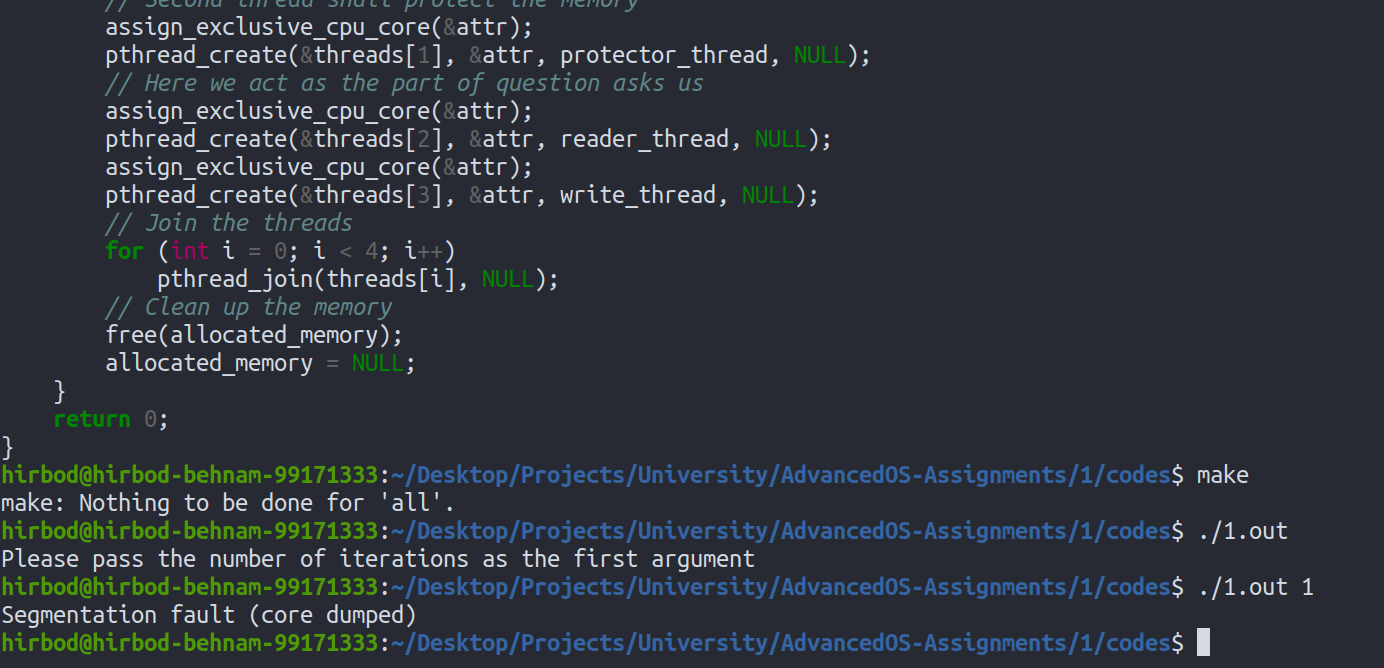
\includegraphics[scale=0.5]{pics/segfault1.png}
    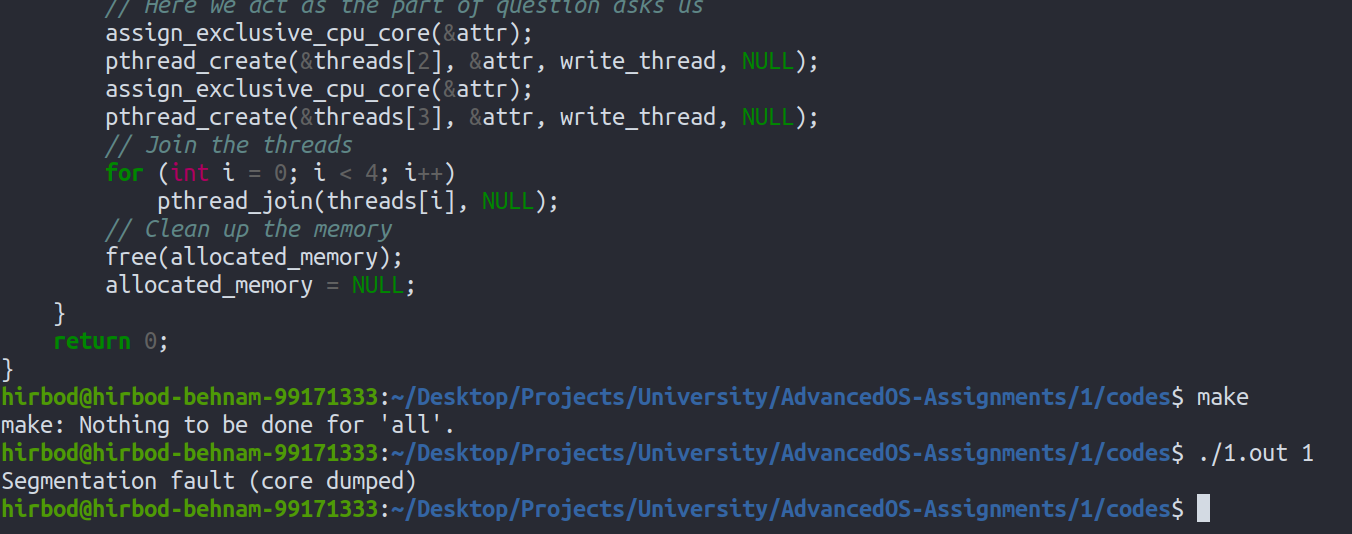
\includegraphics[scale=0.5]{pics/segfault2.png}
\end{figure}

اما در حالتی که دو ترد در حال خواندن هستند مشکلی پیش نمی‌آید.
سپس به کمک \lr{perf}
به ازای تعداد بار‌های مختلف،‌ تعداد
\lr{TLB shootdown}
را اندازه گیری می‌کنیم.